\documentclass[12pt]{report}
\usepackage{graphicx}
\graphicspath{{figure/}}
\usepackage{listings}
\usepackage{xcolor}	%for custom colors in code

\usepackage{titlesec}
\titleformat{\section}{\bfseries\Large}{\thesection}{1em}{}


\lstset{
	basicstyle=\ttfamily\small,         % Font size and type
	keywordstyle=\color{blue},          % Keywords in blue
	commentstyle=\color{green},         % Comments in green
	stringstyle=\color{red},            % Strings in red
	numbers=none,                       % Removes line numbers
	xleftmargin=0pt,                    % Removes left margin
	aboveskip=10pt,                     % Adds space before the code block
	belowskip=10pt                      % Adds space after the code block
}

\usepackage{hyperref}
\hypersetup{colorlinks=true, citecolor=blue, linkcolor=blue, urlcolor=red}

\title{Arduino: Build an I.O.T. Environment Monitor}
\author{A synopsis report submission for the first-year project of\\\\
	Master of Technology in Computer Science and Engineering\\\\\\
	\\By\\
	\\Sameer Dixit(Roll No.: 230216008)\\\\
	\\UNDER THE SUPERVISION OF \\
	\\Dr. Rashi Agarwal\\
	\\Associate Professor\\ 
	\\SUBMITTED TO:\\ 
	\\Dr. B B Sagar (Associate Professor)\\
	\\Dr. Shashwati Banerjea (Associate Professor) }
%\date{Dec 2024}

\begin{document}
	\maketitle
	\begin{figure}[h]
		\centering
		
\includegraphics[scale=0.6]{hbtulogo.png}
		\caption[logo]{DEPARTMENT OF COMPUTER SCIENCE AND ENGINEERING Harcourt Butler Technical University, Kanpur}
		\label{hbtu_logo}
	\end{figure}
	\clearpage
	
	%Project report page 01
	\subsection*{Project Report: Department of Computer Science and Engineering}
	\vspace{0.5cm}
	
	\subsection*{Arduino: Build an IoT Environment Monitor}
	\vspace{0.5cm}
	
	\section*{Introduction}
	\raggedright
	In today's rapidly evolving world, environmental monitoring plays a crucial role in ensuring
	the well-being of our surroundings. This project focuses on building an Internet of Things
	(IoT) environment monitor using Arduino. The device collects data from various sensors
	and transmits it to the cloud for real-time tracking. This project aims to monitor key
	environmental parameters such as temperature, humidity, air quality, and light intensity.\\
	
	\raggedright
	The scope of this project covers the use of Arduino as the hardware platform, interfacing it
	with sensors, and leveraging IoT technology for data transmission and visualization. IoT
	environmental monitors play a significant role in real-time tracking of conditions. On the
	other hand, the cloud computing space is filled with numerous cloud service providers
	(CSPs) that offer varying levels of performance, pricing, and reliability that we will be
	discussing later in our report. Machine learning models provide a powerful tool to rank
	CSPs based on user requirements.\\
	
	\section*{Motivation}
	IoT-based environmental monitoring systems have been explored in various applications,
	from smart homes to industrial systems. Existing solutions primarily focus on temperature
	and humidity monitoring, but recent advancements have incorporated air quality and light
	sensors as well. This project builds on these technologies, offering a cost-effective solution
	with real-time monitoring capabilities.\\
	
	Similarly, cloud service providers play a critical role in delivering infrastructure, platform,
	and software services. A large body of research has focused on comparing CSPs based on
	key performance indicators like cost, reliability, and scalability. Machine learning has
	emerged as a key approach in evaluating CSPs due to its ability to process large datasets and
	identify patterns.\\
	
	Similarly, cloud service providers play a critical role in delivering infrastructure, platform,
	and software services. A large body of research has focused on comparing CSPs based on
	key performance indicators like cost, reliability, and scalability. Machine learning has
	emerged as a key approach in evaluating CSPs due to its ability to process large datasets and
	identify patterns.\\
	
	\section*{Problem Statement}
	\title{\large Cloud Service Providers}
	There are numerous CSPs across the globe with different services, pricing models, and
	infrastructures.\\
	
	The list of major CSPs across the globe. As per Gartner's Magic Quadrant for Cloud
	Infrastructure and Platform Services published in 2021{Get this report: Gartner's Magic Quadrant for Cloud Infrastructure and Platform Services}.\\
	
	%CSPs list
	\begin{enumerate}
		\item Amazon Web Services (AWS),
		\item Microsoft Azure,
		\item Google Cloud Platform (GCP),
		\item IBM Cloud.
	\end{enumerate}
	\vspace{0.2cm}	
	Once the top four vendors are identified, the primary goal is to choose the most appropriate
	one among them for user's software requirement specification.
	
	\paragraph*{Components and Tools:}
	The components and tools used in this project are categorized into hardware and software:
	
	%Hardware list
	\paragraph{Hardware}
	\begin{itemize}
		\item Arduino Uno
		\item DHT11/DHT22 (Temperature and Humidity Sensor)
		\item MQ135 (Air Quality Sensor)
		\item Light Sensor (LDR)
		\item Wi-Fi Module (ESP8266/ESP32)
		\item Jumper Wires and Breadboard
	\end{itemize}
	
	%Software list
	\paragraph{Software}
	\vspace{0.5cm}
	\begin{itemize}
		\item Arduino IDE for coding 
		\item ThingSpeak/Blynk for IoT platform 
		\item APIs for data visualization
	\end{itemize}
	
	
	\vspace{0.5cm}
	\section*{Abstract}
	The system consists of sensors connected to the Arduino board, which processes the data and sends it to an IoT platform via the Wi-Fi module.\\
	
	\vspace*{0.5cm}
	\title{\large Block Diagram\\}
	The block diagram includes sensors (DHT11, MQ135, LDR), Arduino, Wi-Fi module, and the
	cloud for data storage and visualization.\\
	
	\clearpage
	\begin{figure}[h]
		\centering
		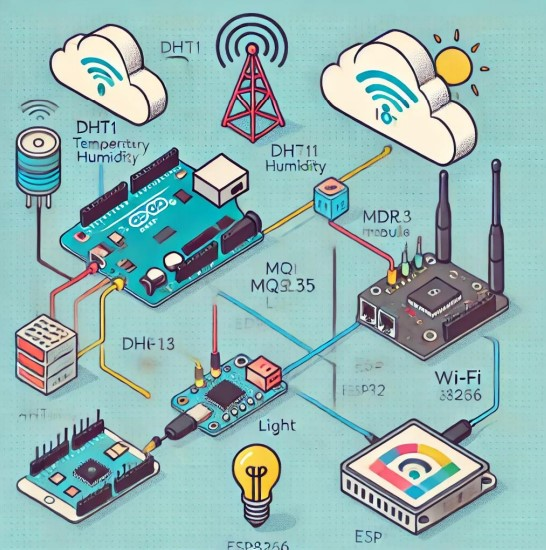
\includegraphics[scale=1]{blockdiagram.jpg}
		\caption[block_fig]{Block Diagram}
		\label{block_fig}
	\end{figure}
	
	
	\section*{Flowchart}
	\subsection*{1. Sensors collect environmental data}
	\begin{figure}[ht]
		\centering
		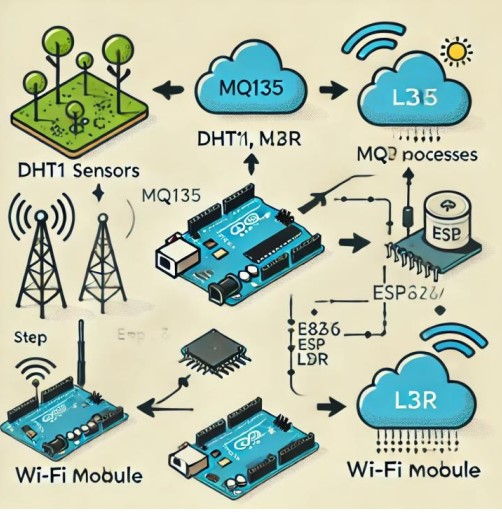
\includegraphics[scale=1]{environmentdata.jpg}
		\caption[environment_fig]{Sensors collect environmental data}
		\label{environment_fig}
	\end{figure}
	
	\subsection*{2. Data is processed by Arduino}
	\begin{figure}[ht]
		\centering
		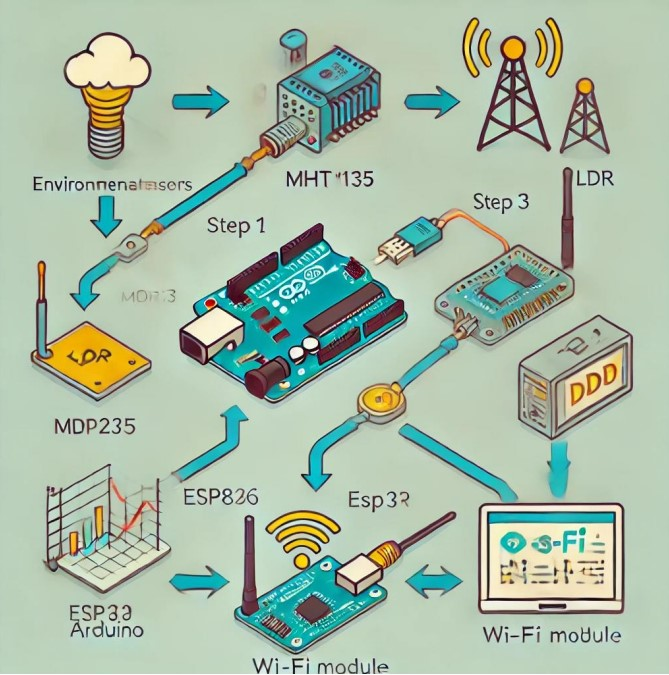
\includegraphics[scale=1]{dataprocess.jpg}
		\caption[data_process]{Data is processed by Arduino}
		\label{data_process}
	\end{figure}
	
	\subsection*{3. Wi-Fi module sends data to the cloud}
	\begin{figure}[ht]
		\centering
		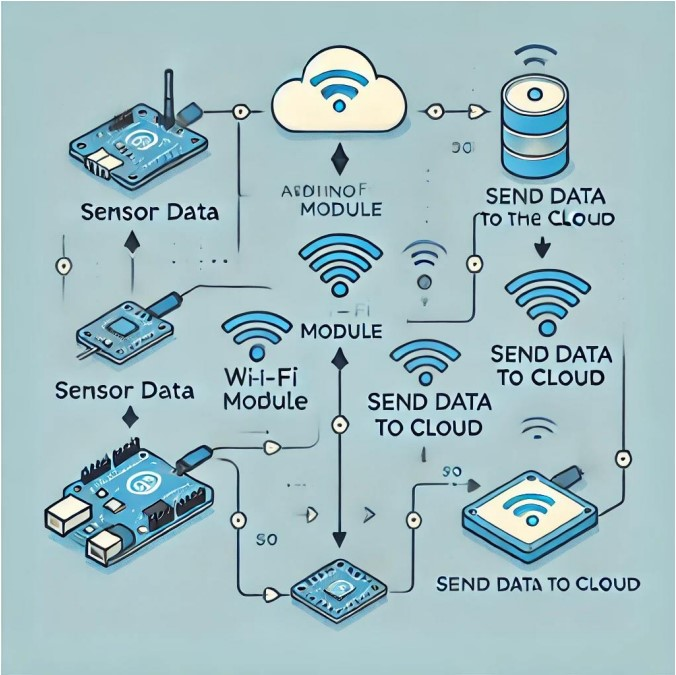
\includegraphics[scale=1]{wifimodel.jpg}
		\caption[wifi_model]{Wi-Fi module sends data to the cloud}
		\label{wifi_model}
	\end{figure}
	
	\subsection*{4. The user accesses the data via an IoT dashboard}
	\begin{figure}[ht]
		\centering
		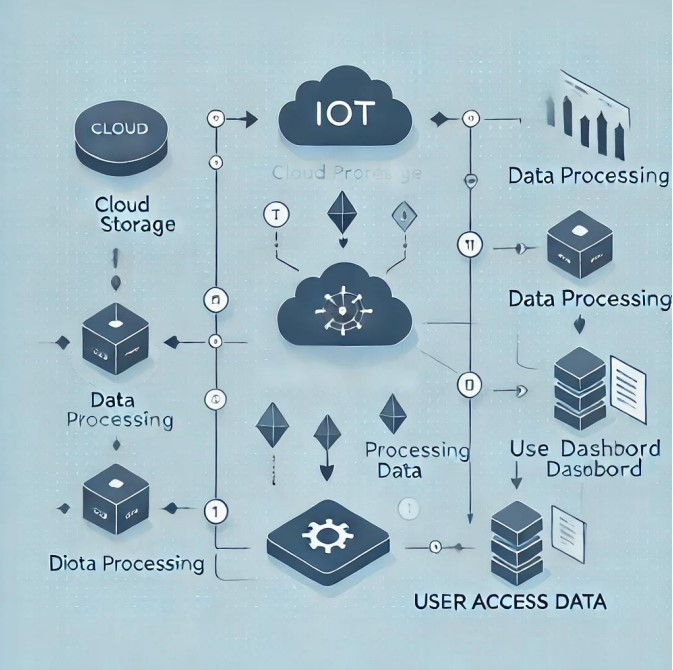
\includegraphics[scale=1]{useraccess.jpg}
		\caption[user_access]{Wi-Fi module sends data to the cloud}
		\label{user_access}
	\end{figure}
	\clearpage
	
	\section{Goals and Objectives with Circuit Design and Assembly}
	The circuit involves connecting the sensors to the respective pins of the Arduino board, and
	setting up the Wi-Fi module for internet connectivity.
	
	\vspace{0.5cm}
	Power is supplied through a USB connection or a dedicated power source, and appropriate
	jumper wires are used to establish connections between the components.
	
	
	\begin{figure}[ht]
		\centering
		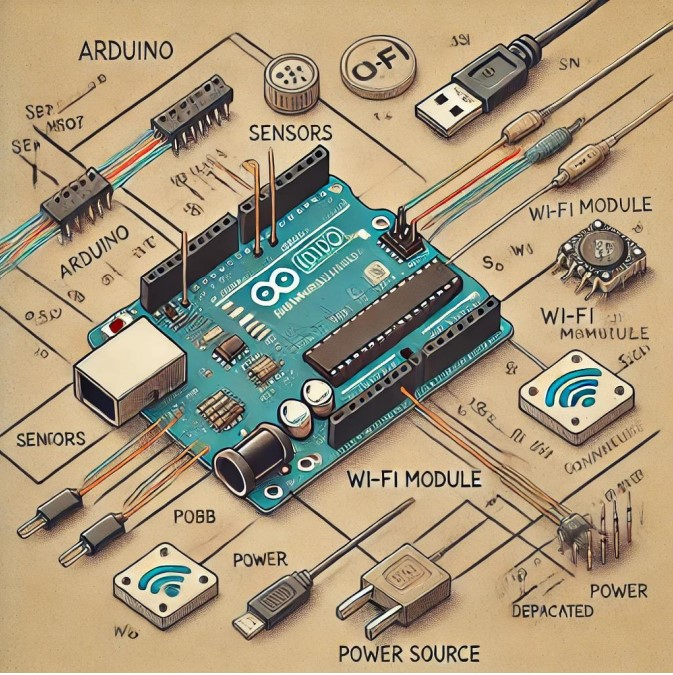
\includegraphics[scale=1]{circuitdesign.jpg}
		\caption[circuit_design]{Circuit Design and Assembly}
		\label{circuit_design}
	\end{figure}
	
	\subsection{Software Implementation}
	The Arduino code initializes the sensors, collects data, and sends it to the IoT platform via
	the Wi-Fi module. Below is a brief code snippet to illustrate how the temperature and
	humidity sensor (DHT11) is initialized.
	
	
	\par
	\noindent
	\begin{lstlisting}[language=C++, caption={DHT11 Code}]
		void setup() {
			Serial.begin(9600);
			dht.begin();
		}
		
		void loop() {
			float humidity = dht.readHumidity();
			float temperature = dht.readTemperature();
		}
		// Send data to cloud
		}
	\end{lstlisting}
	
	
	
	The data collected from the sensors is sent to an IoT platform like ThingSpeak or Blynk. This platform provides real-time monitoring and historical data visualization.\\
	
	\subsection*{Steps to Set Up ThingSpeak/Blynk}
	\begin{enumerate}
		\item Create an account on the platform.
		\item Set up a new channel for data logging.
		\item Configure the Arduino code to send data to the platform using API keys.
	\end{enumerate}
	
	
	\section{Literature Survey and Research Methodology}
	
	\begin{itemize}
		\item \textbf{Wide Detection Range}: It can detect a range of harmful gases, making it suitable for both industrial and domestic applications.
		\item \textbf{Sensitivity}: The sensor provides an analog output corresponding to the concentration of gases, allowing for precise monitoring.
		\item \textbf{Low Cost}: MQ135 is one of the more affordable gas sensors, making it popular for DIY projects, IoT systems, and academic purposes.
		\item \textbf{Durability}: It has a long lifespan and works reliably in various environmental conditions.
		\item \textbf{Easy to Interface}: It can easily be integrated with micro controllers like Arduino, Raspberry Pi, or other IoT platforms via its analog and digital pins.
	\end{itemize}
	
	
	\begin{figure}[ht]
		\centering
		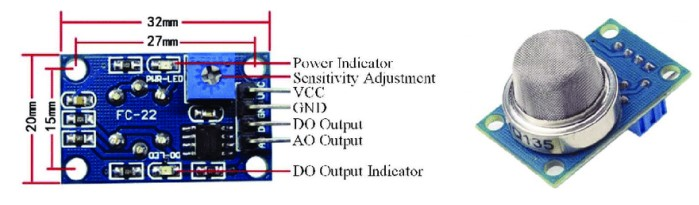
\includegraphics[scale=1.2]{widedetection.jpg}
		\caption[wide_detection]{Key Features and Advantages of the MQ135 Gas Sensor}
		\label{wide_detection}
	\end{figure}
	
	
	\section*{Applications}
	
	\begin{itemize}
		\item \textbf{Air Quality Monitoring}: Commonly used in IoT-based systems to monitor indoor air quality, especially in homes, offices, and schools.
		\item \textbf{Industrial Safety Systems}: Used to detect the presence of harmful gases in factories or workplaces to ensure safety standards.
		\item \textbf{Smart Homes}: Integrated with home automation systems for real-time air quality checks and triggering alarms or ventilation systems if unsafe gas levels are detected.
		\item \textbf{Environmental Monitoring}: Applied in environmental stations to detect pollution levels in urban areas or near industrial zones.
	\end{itemize}
	\clearpage
	
	
	\section*{IoT Cloud Integration}
	The data collected from the sensors is sent to an IoT platform like ThingSpeak or Blynk. This platform provides real-time monitoring and historical data visualization.
	
	\subsection*{Steps to set up ThingSpeak/Blynk:}
	\begin{enumerate}
		\item Create an account on the platform.
		\item Set up a new channel for data logging.
		\item Configure the Arduino code to send data to the platform using API keys.
	\end{enumerate}
	
	\section*{Testing and Results}
	The environment monitor was tested in different conditions to measure temperature, humidity, air quality, and light levels. The following graphs show the data collected during the testing phase, highlighting variations in environmental factors over time.
	
	\begin{figure}[ht]
		\centering
		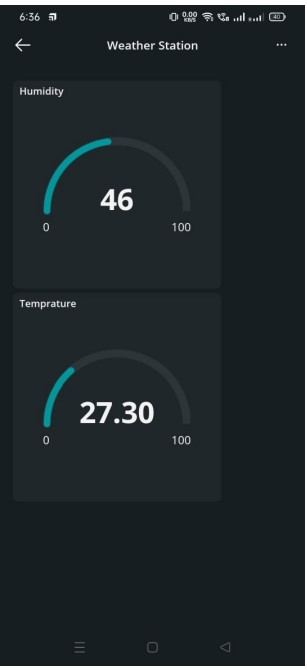
\includegraphics[scale=1.4]{weatherstation.jpg}
		\caption[test_results]{Environmental Data Analysis}
		\label{test_results}
	\end{figure}
	\clearpage
	
	\section*{Applications and Future Scope}
	This project has applications in smart homes, industries, agriculture, and environmental
	research. Future work may include integrating additional sensors (e.g., CO2 sensors) and
	leveraging machine learning for predictive environmental analysis.\\
	\begin{figure}[ht]
		\centering
		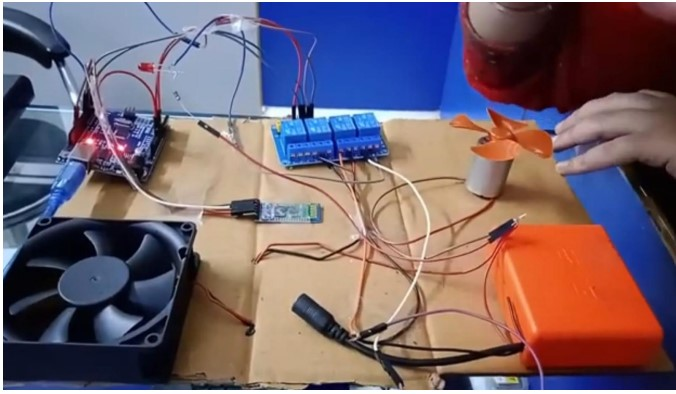
\includegraphics[scale=1.2]{futurescope01.jpg}
		\caption[smart_sol]{Smart solutions for environmental research with future sensor and AI enhancements.}
		\label{smart_sol}
	\end{figure}
	
	\begin{figure}[ht]
		\centering
		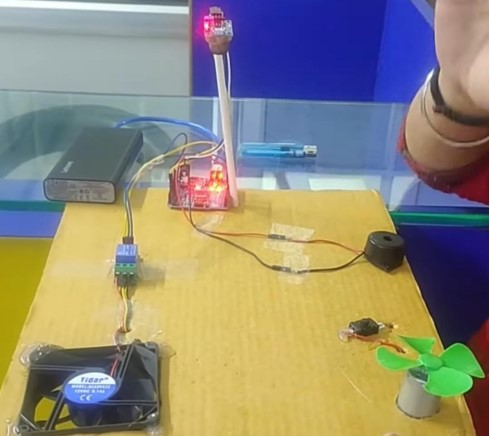
\includegraphics[scale=1.5]{futurescope02.jpg}
		\caption[monitoring]{Environmental monitoring with potential for sensor upgrades and predictive analysis.}
		\label{monitoring}
	\end{figure}
	
	\clearpage
	%Conclusion
	\section*{Conclusion}
	In conclusion, this project successfully demonstrates the integration of Arduino with IoT for real-time environmental monitoring. It offers a cost-effective solution for tracking various environmental parameters and provides significant opportunities for future improvements.
	
	
	
	\end{document}